\chapter{المحركات والآلات الحرارية}\label{ch:b1:heat-engines}

محرك سيارة، ومحطة توليد، \omterm{def:b1:heat-engines:machine}{وثلاجة}، \omterm{def:b1:heat-engines:machine}{ومضخة حرارية}: كلها الشيء
نفسه منظورًا إليه من أربع جهات: مائع يُدار في دور، ويكون
بالتناوب في تماسّ مع منبع ساخن وآخر بارد، فيتبادل الحرارة مع
كليهما والشغل مع عمود. فالمبدأ الأول يمسك حساب الطاقة؛ والمبدأ
الثاني، عبر موازنة الإنتروبيا على امتداد دور واحد، يقيم الحدّ
الذي لا تغلبه براعة --- وهو \omterm{thm:b1:heat-engines:carnot}{مبرهنة كارنو}، أبعد متراجحات هندسة الآلات
أثرًا. ويشتقّ هذا الفصل ذلك الحدّ، ويحسب الدور المثالي والأدوار
الحقيقية التي تقترب منه (أوتو وديزل وستيرلنغ)، ثم يعكس الآلة
لصنع البرد وتدفئة البيوت، ويبيّن كيف تُدفَع إنتروبيا آلة حقيقية
المُنشأة، جولًا بجول، شغلًا ضائعًا.

\section{الآلات الدورية والمبدآن}

\begin{definition}[الآلة الترموديناميكية]\label{def:b1:heat-engines:machine}
\index{محرك حراري}\index{ثلاجة}\index{مضخة حرارية}\index{منظم حراري}
\emph{الآلة الترموديناميكية} \omterm{def:b1:newton-dynamics:conservation}{جملة مغلقة} (هي المائع العامل)
تُدار في \emph{دور}، فتعود دوريًّا إلى الحالة نفسها،
بينما تتبادل الشغل $W$ مع الخارج والحرارة $Q_i$ مع
منابع عند درجات الحرارة $T_i$ --- وهي \emph{منظِّمات حرارية}، لا يغيّر
التبادل درجة حرارتها. والآلة \emph{ثنائية المنبع} تستعمل
منظِّمين حراريين، هما المنبع الساخن عند $T_h$ والمنبع البارد عند $T_c < T_h$.
وتكون \emph{محركًا} إن قدّمت شغلًا ($W < 0$)، و\emph{ثلاجة}
إن أُديرت ($W > 0$) لتأخذ الحرارة من المنبع
البارد، و\emph{مضخة حرارية} إن أُديرت لتعطي الحرارة للمنبع الساخن.
وتُحسب المقادير كلها على امتداد دور واحد، جبريًّا، بوصفها متلقاةً
من المائع.
\end{definition}

\begin{theorem}[المبدآن على امتداد دور؛ متراجحة كلاوزيوس]\label{thm:b1:heat-engines:clausius}
\index{متراجحة كلاوزيوس}
على امتداد دور واحد من آلة ثنائية المنبع، يكون
\[
W + Q_h + Q_c = 0 , \qquad
\frac{Q_h}{T_h} + \frac{Q_c}{T_c} = -S_{\mathrm{created}} \leq 0 ,
\]
مع المساواة في العلاقة الثانية إذا كان الدور عكوسًا وفقط إذا كان
كذلك. وعمومًا، من أجل أيّ عدد من المنظِّمات الحرارية، يكون
$\sum_i Q_i/T_i \leq 0$ (وهي \emph{\omterm{thm:b1:heat-engines:clausius}{متراجحة كلاوزيوس}}).
\end{theorem}

\begin{proof}
$U$ و $S$ دالتا حالة، فيكون $\Delta U = 0$ و $\Delta S = 0$ على امتداد
دور. ويعطي المبدأ الأول $0 = W + Q_h + Q_c$؛ وتعطي موازنة الإنتروبيا
(\cref{thm:b1:second-law-entropy:secondlaw}) أن $0 = S_{\mathrm{exch}} +
S_{\mathrm{created}}$ مع $S_{\mathrm{exch}} = \sum Q_i/T_i$ لأن كل
منظِّم حراري يتبادل عند درجة حرارته الثابتة
(\cref{prop:b1:second-law-entropy:thermostat}).
\end{proof}

\begin{corollary}[كلفن من جديد]\label{cor:b1:heat-engines:kelvin}
الآلة \emph{الأحادية المنبع} ($Q_c = 0$) لها $Q_h \leq 0$، ومنه $W \geq 0$:
فلا يستطيع دور أن يحوّل حرارة منبع واحد إلى شغل. ولا تستطيع
سفينة أن تبحر بتبريد البحر --- فالمحرك يحتاج إلى منبع بارد
يطرح فيه الحرارة، والمبدأ الثاني يقول كم عليه أن يطرح.
\end{corollary}

\begin{omfigure}
\begin{tikzpicture}[font=\small, x=1cm, y=1cm, >=Stealth]
  % engine
  \begin{scope}
    \draw[fill=omThm!15, draw=omThm, thick] (-1.6,3.0) rectangle (1.6,3.7) node[midway] {المنبع الساخن $T_h$};
    \draw[fill=omDef!15, draw=omDef, thick] (-1.6,-0.7) rectangle (1.6,0) node[midway] {المنبع البارد $T_c$};
    \draw[thick, rounded corners, fill=omProp!10] (-0.9,1.0) rectangle (0.9,2.0) node[midway] {المحرك};
    \draw[->, omThm, very thick] (0,3.0) -- (0,2.0) node[midway, right] {$Q_h > 0$};
    \draw[->, omDef, very thick] (0,1.0) -- (0,0) node[midway, right] {$Q_c < 0$};
    \draw[->, omProp, very thick] (0.9,1.5) -- (2.3,1.5) node[midway, above] {$W < 0$};
    \node[font=\footnotesize] at (0,-1.1) {$\eta = -W/Q_h$};
  \end{scope}
  % refrigerator / heat pump
  \begin{scope}[xshift=6.4cm]
    \draw[fill=omThm!15, draw=omThm, thick] (-1.6,3.0) rectangle (1.6,3.7) node[midway] {المنبع الساخن $T_h$};
    \draw[fill=omDef!15, draw=omDef, thick] (-1.6,-0.7) rectangle (1.6,0) node[midway] {المنبع البارد $T_c$};
    \draw[thick, rounded corners, fill=omProp!10] (-1.1,1.0) rectangle (1.1,2.0) node[midway, align=center, font=\footnotesize] {ثلاجة\\ أو مضخة حرارية};
    \draw[->, omThm, very thick] (0,2.0) -- (0,3.0) node[midway, right] {$Q_h < 0$};
    \draw[->, omDef, very thick] (0,0) -- (0,1.0) node[midway, right] {$Q_c > 0$};
    \draw[->, omProp, very thick] (-2.5,1.5) -- (-1.1,1.5) node[midway, above] {$W > 0$};
    \node[font=\footnotesize] at (0,-1.1) {$e_f = Q_c/W$, \quad $e_p = -Q_h/W$};
  \end{scope}
\end{tikzpicture}

{\small الجهتان اللتان يُدار فيهما دور ثنائي المنبع. على اليمين:
يأخذ المحرك الحرارة من المنبع الساخن، ويطرح جزءًا منها إلى البارد
ويقدّم الفرق شغلًا. وعلى اليسار: الآلة نفسها مُدارة إلى الوراء
تضخّ الحرارة من البارد إلى الساخن؛ فهي \omterm{def:b1:heat-engines:machine}{ثلاجة} إن أُريد $Q_c$، \omterm{def:b1:heat-engines:machine}{ومضخة
حرارية} إن أُريد $|Q_h|$.}
\end{omfigure}

\section{مبرهنة كارنو}

\begin{definition}[المردود ومعاملا الأداء]\label{def:b1:heat-engines:efficiency}
\index{مردود!محرك حراري}\index{معامل الأداء}
\emph{مردود} محرك هو الشغل المقدَّم لواحدة الحرارة
المأخوذة من المنبع الساخن، $\eta = -W/Q_h$؛ و\emph{معامل
الأداء} \omterm{def:b1:heat-engines:machine}{لثلاجة} هو البرد
المنتَج لواحدة الشغل، $e_f = Q_c/W$؛ وهو \omterm{def:b1:heat-engines:machine}{لمضخة حرارية} الحرارة
المقدَّمة لواحدة الشغل، $e_p = -Q_h/W$. وكلٌّ منها نسبة ``ما يريده
المرء'' إلى ``ما يدفعه''؛ ولا يتجاوز المردود~1، أما معامل الأداء فقد
يتجاوز~1.
\end{definition}

\begin{theorem}[كارنو]\label{thm:b1:heat-engines:carnot}
\index{مبرهنة كارنو}\index{مردود كارنو}
بين منظِّمين حراريين $T_h > T_c$، يكون
\[
\eta \leq \eta_C = 1 - \frac{T_c}{T_h}, \qquad
e_f \leq \frac{T_c}{T_h - T_c}, \qquad
e_p \leq \frac{T_h}{T_h - T_c} = 1 + \frac{T_c}{T_h - T_c},
\]
مع المساواة إذا كان الدور عكوسًا وفقط إذا كان كذلك. ولا تتوقف
الحدود إلا على درجات الحرارة --- لا على المائع ولا على الآلية.
\end{theorem}

\begin{proof}
من أجل محرك ($Q_h > 0$): $\eta = -W/Q_h = (Q_h + Q_c)/Q_h = 1 + Q_c/Q_h$،
وتعطي \omterm{thm:b1:heat-engines:clausius}{متراجحة كلاوزيوس} أن $Q_c/Q_h \leq -T_c/T_h$. ومن أجل
\omterm{def:b1:heat-engines:machine}{ثلاجة} ($Q_c > 0$ و $W > 0$): $W = -Q_h - Q_c$ مع $-Q_h \geq Q_c T_h/T_c$،
ومنه $W \geq Q_c(T_h/T_c - 1)$ و $e_f = Q_c/W \leq T_c/(T_h - T_c)$.
وللمضخة الحرارية: $e_p = -Q_h/W = (W + Q_c)/W = 1 + e_f$. والمساواة هي
الحالة العكوسة $S_{\mathrm{created}} = 0$ في كل موضع.
\end{proof}

\begin{example}[ثلاثة أعداد]\label{ex:b1:heat-engines:numbers}
عنفة بخارية بين $T_h = \qty{800}{K}$ ونهر عند
$T_c = \qty{300}{K}$: $\eta_C = 0.625$؛ وتبلغ المحطات الحقيقية نحو $0.40$.
\omterm{def:b1:heat-engines:machine}{وثلاجة} منزلية بين $\qty{275}{K}$ في الداخل ومطبخ عند
$\qty{298}{K}$: $e_f \leq 275/23 = 12$؛ وتعطي الآلات الحقيقية $2$ إلى $4$.
\omterm{def:b1:heat-engines:machine}{ومضخة حرارية} تدفئ بيتًا عند $\qty{293}{K}$ من هواء عند $\qty{273}{K}$:
$e_p \leq 293/20 = 14.7$؛ وتعطي المضخات الحقيقية $3$ إلى $5$ --- أي ثلاثة
إلى خمسة أضعاف ما كانت الكهرباء نفسها لتعطيه في مقاومة
(\cref{pb:b1:heat-engines:1}).
\end{example}

\begin{remark}[لماذا لا يبلغ المردود~1]\label{rem:b1:heat-engines:why}
يتلقى المحرك الإنتروبيا $Q_h/T_h$ مع الحرارة التي يأخذها؛ ولا يحمل
الشغل منها شيئًا؛ فلا مخرج إلا الحرارة المطروحة إلى المنبع البارد،
وهي تحمل $|Q_c|/T_c$. وما دامت الإنتروبيا لا تُفنى، وجب طرح
$Q_h T_c/T_h$ على الأقل من الحرارة، ويكون الشغل ما يتبقى.
فكلما انخفض المنبع البارد وارتفع الساخن كان أفضل --- ومن هنا
أبراج التبريد، والسعي وراء ريش عنفات أشدّ حرارة أبدًا.
\end{remark}

\section{دور كارنو}

\begin{definition}[دور كارنو]\label{def:b1:heat-engines:carnotcycle}
\index{دور كارنو}
\emph{دور كارنو} هو الدور العكوس الثنائي المنبع: متساويا حرارة
عكوسان، عند $T_h$ (في تماسّ مع المنبع الساخن) وعند $T_c$ (مع
البارد)، يصل بينهما ساقان كظومان عكوسان (متساويا الإنتروبيا،
بلا تماسّ مع منبع). فإذا أُدير مع عقارب الساعة في المستوي $(V, P)$ كان
محركًا؛ وإذا أُدير عكسها كان \omterm{def:b1:heat-engines:machine}{ثلاجة} أو \omterm{def:b1:heat-engines:machine}{مضخة حرارية}. وفي \omterm{def:b1:second-law-entropy:TS}{مخطط
الإنتروبيا} يكون مستطيلًا.
\end{definition}

\begin{proposition}[دور كارنو لغاز مثالي]\label{prop:b1:heat-engines:carnotgas}
من أجل $n$ مولًا من \omterm{def:b1:kinetic-theory:model}{غاز مثالي} يُدار على $A \to B$ (متساوي حرارة $T_h$،
تمدد) ثم $B \to C$ (كظوم) ثم $C \to D$ (متساوي حرارة $T_c$،
انضغاط) ثم $D \to A$ (كظوم):
\[
Q_h = nRT_h\ln\frac{V_B}{V_A}, \qquad
Q_c = -nRT_c\ln\frac{V_B}{V_A}, \qquad
\eta = 1 - \frac{T_c}{T_h} ,
\]
وهي قيمة كارنو --- كما يجب أن تكون من أجل أيّ دور عكوس ثنائي المنبع.
\end{proposition}

\begin{proof}
على متساوي الحرارة يكون $\Delta U = 0$، ومنه $Q = -W = nRT\ln(V_{\text{النهائي}}/
V_{\text{الابتدائي}})$. وعلى الكظومين يكون $TV^{\gamma-1}$ ثابتًا:
$T_hV_B^{\gamma-1} = T_cV_C^{\gamma-1}$ و $T_hV_A^{\gamma-1} =
T_cV_D^{\gamma-1}$، ومنه $V_C/V_D = V_B/V_A$ و $Q_c = nRT_c\ln(V_D/V_C) =
-nRT_c\ln(V_B/V_A)$. ثم $\eta = 1 + Q_c/Q_h = 1 - T_c/T_h$.
\end{proof}

\begin{omfigure}
\begin{tikzpicture}
\begin{axis}[omaxis, axis x line=bottom, axis y line=left, width=7.6cm, height=5.6cm,
    xlabel={$V$}, ylabel={$P$}, xmin=0, xmax=6.3, ymin=0, ymax=1.7,
    xlabel style={at={(axis description cs:0.5,-0.06)}, anchor=north},
    xtick=\empty, ytick=\empty, samples=60]
  \addplot[omThm, thick, domain=1:2] {1.5/x} node[pos=0.5, above right, font=\footnotesize] {$T_h$};
  \addplot[omProp, thick, domain=2:5.51] {0.75*(2/x)^1.4};
  \addplot[omDef, thick, domain=2.756:5.51] {1/x} node[pos=0.2, below left, font=\footnotesize] {$T_c$};
  \addplot[omProp, thick, domain=1:2.756] {0.3628*(2.756/x)^1.4};
  \node[font=\footnotesize, anchor=south west] at (axis cs:0.95,1.52) {$A$};
  \node[font=\footnotesize, anchor=south west] at (axis cs:2.05,0.77) {$B$};
  \node[font=\footnotesize, anchor=north west] at (axis cs:5.5,0.18) {$C$};
  \node[font=\footnotesize, anchor=north east] at (axis cs:2.7,0.35) {$D$};
  \node[font=\footnotesize, omProp] at (axis cs:4.4,0.62) {كظومان};
  \draw[-Stealth, thick] (axis cs:1.45,1.1) -- (axis cs:1.55,1.0);
  \draw[-Stealth, thick] (axis cs:4.3,0.22) -- (axis cs:4.1,0.235);
\end{axis}
\end{tikzpicture}\hfill
\begin{tikzpicture}
\begin{axis}[omaxis, axis x line=bottom, axis y line=left, width=6.2cm, height=5.6cm,
    xlabel={$S$}, ylabel={$T$}, xmin=-1.2, xmax=4.6, ymin=0, ymax=2.2, clip=false,
    xlabel style={at={(axis description cs:0.5,-0.1)}, anchor=north},
    xtick={1,3}, xticklabels={$S_1$,$S_2$}, ytick={0.8,1.6}, yticklabels={$T_c$,$T_h$}]
  \fill[omProp!20] (axis cs:1,0.8) rectangle (axis cs:3,1.6);
  \draw[omThm, thick, -Stealth] (axis cs:1,1.6) -- (axis cs:3,1.6) node[midway, above, font=\footnotesize] {$A \to B$};
  \draw[omProp, thick, -Stealth] (axis cs:3,1.6) -- (axis cs:3,0.8) node[midway, right, font=\footnotesize] {$B \to C$};
  \draw[omDef, thick, -Stealth] (axis cs:3,0.8) -- (axis cs:1,0.8) node[midway, below, font=\footnotesize] {$C \to D$};
  \draw[omProp, thick, -Stealth] (axis cs:1,0.8) -- (axis cs:1,1.6) node[midway, left, font=\footnotesize] {$D \to A$};
  \node[font=\footnotesize] at (axis cs:2,1.2) {$-W$};
\end{axis}
\end{tikzpicture}

{\small \omterm{def:b1:heat-engines:carnotcycle}{دور كارنو} \omterm{def:b1:kinetic-theory:model}{لغاز مثالي}. على اليمين: في مخطط
كلابيرون متساويا حرارة وكظومان (أشدّ ميلًا)، يُدار مع عقارب الساعة؛
والمساحة المحصورة هي الشغل المقدَّم. وعلى اليسار: الدور نفسه في
\omterm{def:b1:second-law-entropy:TS}{مخطط الإنتروبيا} مستطيل ارتفاعه $T_h - T_c$ وعرضه
$Q_h/T_h$؛ ومساحته هي $-W$ من جديد، ونسبة تلك المساحة إلى
المساحة تحت ضلعه العلوي، $Q_h$، هي $1 - T_c/T_h$ بمجرد النظر.}
\end{omfigure}

\begin{remark}[دور كارنو مبرهنة لا محرك]\label{rem:b1:heat-engines:notengine}
تقتضي متساويات الحرارة العكوسة نقلًا للحرارة بطيئًا إلى ما لا نهاية عبر
فرق متلاشٍ في \omterm{def:b1:kinetic-theory:temperature}{درجة الحرارة}: فمحرك كارنو يقدّم شغله الأعظمي
عند استطاعة معدومة. وتقايض الآلات الحقيقية المردودَ بالاستطاعة بقبول
فروق منتهية في درجات الحرارة داخل مبادلاتها
(\cref{exo:b1:heat-engines:10})؛ وتبقى قيمة كارنو السقف الذي
يُقاس به كل تصميم.
\end{remark}

\section{أدوار المحركات الحقيقية}

\begin{proposition}[دور أوتو]\label{prop:b1:heat-engines:otto}
\index{دور أوتو}\index{نسبة الانضغاط}
يدير محرك البنزين المثالي الهواء ($\gamma$) على: $1 \to 2$
انضغاط كظوم من $V_1$ إلى $V_2$ (و\emph{\omterm{prop:b1:heat-engines:otto}{نسبة الانضغاط}}
$r = V_1/V_2$)؛ ثم $2 \to 3$ تسخين متساوي الحجم (هو الاحتراق)؛ ثم $3 \to 4$
تمدد كظوم عائد إلى $V_1$؛ ثم $4 \to 1$ تبريد متساوي الحجم (هو
العادم). ومردوده هو
\[
\eta_{\text{أوتو}} = 1 - \frac{1}{r^{\gamma-1}} .
\]
\end{proposition}

\begin{proof}
لا تُتبادَل الحرارة إلا على متساويَي الحجم: $Q_h = nC_{V,m}(T_3 - T_2)$ و
$Q_c = nC_{V,m}(T_1 - T_4)$. وعلى الكظومين يكون $TV^{\gamma-1}$ ثابتًا:
$T_2 = T_1r^{\gamma-1}$ و $T_3 = T_4r^{\gamma-1}$، ومنه $T_3 - T_2 =
(T_4 - T_1)r^{\gamma-1}$ و
$\eta = 1 + Q_c/Q_h = 1 - (T_4 - T_1)/(T_3 - T_2) = 1 - r^{1-\gamma}$.
\end{proof}

\begin{example}[أعداد لمحرك بنزين]\label{ex:b1:heat-engines:ottonumbers}
مع $r = 9$ و $\gamma = 1.4$: $9^{0.4} = 2.41$ و $\eta = 0.58$. ويعطي محرك حقيقي
نحو $0.30$: فالاحتراق ليس لحظيًّا، والغاز ليس
مثاليًّا عند \qty{2500}{K}، والحرارة تتسرب إلى الجدران، والاحتكاك والضخّ
يأخذان نصيبهما. ورفع $r$ يفيد --- إلى أن يشتعل مزيج الهواء والوقود
من تلقائه في نهاية الانضغاط (وهو الطرق)؛ ومحرك الديزل
يحوّل تلك الرذيلة إلى مبدأ له.
\end{example}

\begin{proposition}[دور ديزل]\label{prop:b1:heat-engines:diesel}
\index{دور ديزل}
استبدل بالتسخين المتساوي الحجم في \omterm{prop:b1:heat-engines:otto}{دور أوتو} تسخينًا متساوي الضغط، من
$V_2$ إلى $V_3 = \rho V_2$ (و\emph{نسبة القطع} $\rho > 1$): فالوقود المحقون
في هواء صار ساخنًا بنسبة انضغاط $r$ من $15$ إلى $22$ يحترق
لحظة وصوله. وعندئذ
\[
\eta_{\text{ديزل}} = 1 - \frac{1}{r^{\gamma-1}}\,\frac{\rho^{\gamma} - 1}{\gamma(\rho - 1)} ,
\]
وهو أصغر من قيمة أوتو عند $r$ نفسها لكنه يُبلَغ بنسبة انضغاط $r$ أكبر بكثير،
فيكون أكبر عمليًّا ($0.40$ إلى $0.45$ في المحركات الكبيرة).
\end{proposition}

\begin{proof}
لدينا $Q_h = nC_{P,m}(T_3 - T_2)$ و $Q_c = nC_{V,m}(T_1 - T_4)$، ومنه $\eta = 1 -
(T_4 - T_1)/[\gamma(T_3 - T_2)]$. ومع $T_2 = T_1r^{\gamma-1}$ و $T_3 =
\rho T_2$، وعلى الكظوم $3 \to 4$ (حيث $V_4 = V_1 = rV_2$)، يكون $T_4 =
T_3(V_3/V_4)^{\gamma-1} = \rho T_1 r^{\gamma-1}(\rho/r)^{\gamma-1} = T_1\rho^{\gamma}$:
ومنه $\eta = 1 - (\rho^\gamma - 1)/[\gamma r^{\gamma-1}(\rho - 1)]$.
\end{proof}

\begin{omfigure}
\begin{tikzpicture}
\begin{axis}[omaxis, axis x line=bottom, axis y line=left, width=7.2cm, height=5.6cm,
    xlabel={$V$}, ylabel={$P$}, xmin=0, xmax=5.6, ymin=0, ymax=15.5, clip=false,
    xlabel style={at={(axis description cs:0.5,-0.06)}, anchor=north},
    xtick={1,4}, xticklabels={$V_2$,$V_1$}, ytick=\empty, samples=60]
  \addplot[omProp, thick, domain=1:4] {x^(-1.4)*6.96};
  \addplot[omThm, very thick] coordinates {(1,6.96) (1,13.9)};
  \addplot[omProp, thick, domain=1:4] {13.9*x^(-1.4)};
  \addplot[omDef, very thick] coordinates {(4,2.0) (4,1)};
  \node[font=\footnotesize, anchor=north east] at (axis cs:3.95,0.95) {$1$};
  \node[font=\footnotesize, anchor=east] at (axis cs:0.9,6.96) {$2$};
  \node[font=\footnotesize, anchor=south west] at (axis cs:1.05,13.9) {$3$};
  \node[font=\footnotesize, anchor=south west] at (axis cs:4.05,2.1) {$4$};
  \node[font=\footnotesize, omThm, anchor=west] at (axis cs:1.15,10.5) {$Q_h$ (الاحتراق)};
  \node[font=\footnotesize, omDef, anchor=west] at (axis cs:4.15,1.0) {$Q_c$ (العادم)};
  \draw[-Stealth, thick] (axis cs:2.0,5.25) -- (axis cs:2.2,4.6);
  \draw[-Stealth, thick] (axis cs:2.2,2.33) -- (axis cs:2.0,2.65);
  \node[font=\footnotesize, omProp, anchor=west] (lblexp) at (axis cs:2.9,6.4) {تمدد};
  \draw[omProp, -Stealth] (lblexp.west) -- (axis cs:2.55,3.9);
  \node[font=\footnotesize, omProp, anchor=west] (lblcomp) at (axis cs:4.4,4.6) {انضغاط};
  \draw[omProp, -Stealth] (lblcomp.west) -- (axis cs:3.3,1.45);
\end{axis}
\end{tikzpicture}\hfill
\begin{tikzpicture}
\begin{axis}[omaxis, axis x line=bottom, axis y line=left, width=6.6cm, height=5.6cm,
    xlabel={$r$}, ylabel={$\eta$}, xmin=0, xmax=22, ymin=0, ymax=1.05,
    xlabel style={at={(axis description cs:0.5,-0.12)}, anchor=north},
    xtick={5,10,15,20}, ytick={0.2,0.4,0.6,0.8,1}, samples=80]
  \addplot[omThm, thick, domain=1:22] {1-x^(-0.4)} node[pos=0.55, above, font=\footnotesize] {أوتو، $\gamma = 1.4$};
  \addplot[omDef, thick, domain=1.5:22] {1-(2^1.4-1)/(1.4*x^0.4*(2-1))} node[pos=0.415, below right, font=\footnotesize, align=left] {ديزل،\\ $\rho = 2$};
  \addplot[omProp, dashed, thick] coordinates {(9,0) (9,0.585)};
  \addplot[omProp, dashed, thick] coordinates {(18,0) (18,0.632)};
\end{axis}
\end{tikzpicture}

{\small على اليمين: \omterm{prop:b1:heat-engines:otto}{دور أوتو} في مخطط كلابيرون (مرسومًا من أجل $r = 4$): كظومان
ومتساويا حجم؛ وتدخل الحرارة عند النقطة الميتة العليا
وتخرج مع العادم. وعلى اليسار: المردودات المثالية بدلالة
\omterm{prop:b1:heat-engines:otto}{نسبة الانضغاط}؛ ويعلّم الخطان المتقطعان محرك بنزين ($r = 9$) ومحرك
ديزل ($r = 18$ و $\rho = 2$).}
\end{omfigure}

\begin{proposition}[دور ستيرلنغ والمُجدِّد]\label{prop:b1:heat-engines:stirling}
\index{دور ستيرلنغ}\index{مجدد حراري}
متساويا حرارة ($T_c$ و $T_h$) يصل بينهما متساويا حجم. وحرارة
الساقين المتساويي الحجم، $\pm nC_{V,m}(T_h - T_c)$، متساوية ومتعاكسة؛ فإذا
خُزّنت على ساق التبريد في \emph{مُجدِّد} (وهو كتلة مسامية يجري
الغاز خلالها) ورُدّت على ساق التسخين، لم يتبادل مع المنابع
إلا متساويا الحرارة، وكان $\eta = 1 - T_c/T_h$: فمحرك ستيرلنغ
محرك كارنو في كل شيء إلا شكل دوره. وبلا المُجدِّد يجب
أن تأتي حرارة متساويي الحجم من المنبع الساخن ويكون
$\eta = \dfrac{nR(T_h - T_c)\ln(V_1/V_2)}{nRT_h\ln(V_1/V_2) + nC_{V,m}(T_h - T_c)}$،
وهو أدنى بكثير (\cref{exo:b1:heat-engines:8}).
\end{proposition}

\begin{proof}
على متساويي الحرارة يكون $Q_h = nRT_h\ln(V_1/V_2)$ و $Q_c = -nRT_c\ln(V_1/V_2)$، ومنه
$-W = Q_h + Q_c + 0$ متى تلاشت حرارتا متساويي الحجم؛ ثم اقسم على الحرارة
المأخوذة فعلًا من المنبع الساخن في كل حالة.
\end{proof}

\begin{remark}[العنفات البخارية والغازية]\label{rem:b1:heat-engines:turbines}
لا تستعمل محطات التوليد غازًا في أسطوانة، بل ماءً يُغلى،
ويتمدد عبر عنفة، ثم يُكثَّف ويُضخّ عائدًا (وهو دور
رانكين، بتغيّرَي طور --- \cref{ch:b1:phase-changes})، أو هواءً
يُضغط ويُسخَّن بالاحتراق ويتمدد في عنفة غازية (وهو
دور برايتون، بكظومين ومتساويَي ضغط). ويحتاج تحليلها إلى
موازنة الطاقة لمائع جارٍ، وهي في مجلد السنة الثانية؛ أما
حدّ كارنو ومنطق هذا الفصل فينطبقان بلا تغيير.
\end{remark}

\section{الثلاجات والمضخات الحرارية}

\begin{definition}[دور ضغط البخار]\label{def:b1:heat-engines:vapourcycle}
\index{دور ضغط البخار}\index{مائع مبرِّد}
تكاد كل \omterm{def:b1:heat-engines:machine}{ثلاجة} ومجمّد ومكيّف \omterm{def:b1:heat-engines:machine}{ومضخة حرارية} تدير
\emph{مائعًا مبرِّدًا} على أربعة مكوّنات: \emph{ضاغط}
(يتلقى الشغل، ويرفع ضغط البخار)، و\emph{مكثِّف}
(يتسيّل فيه البخار الساخن عند ضغط مرتفع، فيطلق
$|Q_h|$ إلى الجهة الساخنة)، و\emph{صمام تمدد} (يهبط فيه السائل إلى
ضغط منخفض بلا شغل ولا حرارة، ويتبخر بعضه فجأةً)، و\emph{مبخِّر}
(يغلي فيه ما بقي عند ضغط منخفض، فيمتصّ $Q_c$ من
الجهة الباردة). وتُحمَل الحرارة حرارةً كامنة للتبخر،
ويعيّن الضغطان درجتَي الغليان
(\cref{ch:b1:phase-changes}).
\end{definition}

\begin{omfigure}
\begin{tikzpicture}[font=\small, x=1cm, y=1cm, >=Stealth, box/.style={draw, thick, rounded corners, minimum width=2.3cm, minimum height=0.8cm, align=center}]
  \node[box, fill=omThm!12] (cond) at (0,2.2) {مكثِّف\\ \footnotesize ضغط $P$ مرتفع، $T_{\mathrm{cd}}$};
  \node[box, fill=omDef!12] (evap) at (0,-2.2) {مبخِّر\\ \footnotesize ضغط $P$ منخفض، $T_{\mathrm{ev}}$};
  \node[box, fill=omProp!12] (comp) at (3.4,0) {ضاغط};
  \node[box, fill=omExo!12] (valve) at (-3.4,0) {صمام\\ تمدد};
  \draw[->, thick] (evap.east) -| (comp.south) node[pos=0.75, right, font=\footnotesize] {بخار};
  \draw[->, thick] (comp.north) |- (cond.east) node[pos=0.25, right, font=\footnotesize] {بخار ساخن};
  \draw[->, thick] (cond.west) -| (valve.north) node[pos=0.75, left, font=\footnotesize] {سائل};
  \draw[->, thick] (valve.south) |- (evap.west) node[pos=0.25, left, font=\footnotesize] {سائل وبخار};
  \draw[->, omThm, very thick] (cond.north) -- ++(0,0.8) node[above, font=\footnotesize] {$|Q_h|$ إلى الجهة الساخنة ($T_h < T_{\mathrm{cd}}$)};
  \draw[->, omDef, very thick] (0,-3.8) node[below, font=\footnotesize] {$Q_c$ من الجهة الباردة ($T_c > T_{\mathrm{ev}}$)} -- (evap.south);
  \draw[->, omProp, very thick] (5.6,0) node[right, font=\footnotesize] {$W$} -- (comp.east);
\end{tikzpicture}

{\small \omterm{def:b1:heat-engines:vapourcycle}{دور ضغط البخار}. يغلي \omterm{def:b1:heat-engines:vapourcycle}{المائع المبرِّد} في
المبخِّر، وهو أبرد من الجهة الباردة، ويتكثف في المكثِّف،
وهو أسخن من الجهة الساخنة: فتجري الحرارة في اتجاهها الطبيعي عبر كل
مبادل، ويدفع الضاغط ثمن رفعها من
$T_{\mathrm{ev}}$ إلى $T_{\mathrm{cd}}$.}
\end{omfigure}

\begin{proposition}[ثمن فروق درجات الحرارة]\label{prop:b1:heat-engines:gaps}
آلة عكوسة تعمل بين درجتَي حرارتها الداخليتين
$T_{\mathrm{ev}} < T_c$ و $T_{\mathrm{cd}} > T_h$ لها $e_p = T_{\mathrm{cd}}/(T_{\mathrm{cd}} - T_{\mathrm{ev}})$،
وهو أصغر من قيمة كارنو بين المنبعين؛ ولا تبلغ آلة حقيقية
إلا جزءًا (من $0.4$ إلى $0.6$ عادةً) حتى من ذلك. ومن ثمّ يهبط
أداء \omterm{def:b1:heat-engines:machine}{مضخة حرارية} كلما انخفضت \omterm{def:b1:kinetic-theory:temperature}{درجة الحرارة} الخارجية
وارتفعت \omterm{def:b1:kinetic-theory:temperature}{درجة الحرارة} التي تطلبها دارة التدفئة.
\end{proposition}

\begin{proof}
طبّق \cref{thm:b1:heat-engines:carnot} على المائع، الذي تكون
منظِّماته الحرارية فعليًّا درجتَي حرارة المبادلين؛ وكون $T_{\mathrm{cd}} - T_{\mathrm{ev}} >
T_h - T_c$ يخفض النسبة.
\end{proof}

\begin{omfigure}
\begin{tikzpicture}
\begin{axis}[omaxis, axis x line=bottom, axis y line=left, width=10cm, height=7cm,
    xlabel={درجة الحرارة الخارجية (\unit{\degreeCelsius})}, ylabel={$e_p$},
    xlabel style={at={(axis description cs:0.5,-0.08)}, anchor=north},
    xmin=-21, xmax=16, ymin=0, ymax=16, xtick={-20,-10,0,10}, ytick={2,4,...,14}, samples=80, clip=false]
  \addplot[omThm, thick, domain=-20:1.5] {293/(20-x)};
  \node[omThm, font=\footnotesize, anchor=west] at (axis cs:-20,13.9) {كارنو، البيت والهواء الخارجي};
  \addplot[omDef, thick, domain=-20:15] {313/(321-(273+x))};
  \node[omDef, font=\footnotesize, anchor=south east] at (axis cs:15.5,10.3) {كارنو مع فروق المبادلين};
  \addplot[omProp, thick, domain=-20:15] {0.55*313/(321-(273+x))};
  \node[omProp, font=\footnotesize, anchor=south west] at (axis cs:-19.5,3.1) {آلة حقيقية};
  \addplot[black, dashed] coordinates {(-21,1) (16,1)} node[pos=0.9, above, font=\footnotesize] {مقاومة};
\end{axis}
\end{tikzpicture}

{\small معامل أداء \omterm{def:b1:heat-engines:machine}{مضخة حرارية} بدلالة \omterm{def:b1:kinetic-theory:temperature}{درجة الحرارة}
الخارجية: حدّ كارنو بين البيت (\qty{20}{\degreeCelsius}) والهواء
الخارجي؛ والحدّ بعد حساب فروق درجات حرارة المبادلين
($T_{\mathrm{cd}} = \qty{313}{K}$ و $T_{\mathrm{ev}} = T_{\mathrm{out}} - \qty{8}{K}$)؛
وآلة واقعية عند $0.55$ من الأخير. وحتى عند \qty{-10}{\degreeCelsius} تقدّم المضخة الحقيقية نحو
ثلاثة جولات من الحرارة لكل جول من الكهرباء، حيث تعطي المقاومة
جولًا واحدًا.}
\end{omfigure}

\begin{example}[مضخة حرارية أم مقاومة؟]\label{ex:b1:heat-engines:hpvsresistor}
بيت يفقد \qty{6}{kW} عند \qty{-5}{\degreeCelsius} في الخارج يحتاج إلى
\qty{6}{kW} من الكهرباء بالمقاومات؛ وكانت \omterm{def:b1:heat-engines:machine}{مضخة حرارية} مثالية من
\qty{268}{K} إلى \qty{293}{K} لتحتاج إلى $6/11.7 = \qty{0.51}{kW}$؛ أما
الحقيقية بدرجتَي حرارة مبادلين \qty{260}{K} و\qty{313}{K} وبعامل
جودة $0.55$، فمعامل أدائها $e_p = 0.55 \times 313/53 = 3.2$، وتحتاج إلى \qty{1.9}{kW}.
وتجري مسألة نهاية الأسبوع الموسم كله، بالإنتروبيا أيضًا.
\end{example}

\section{الإنتروبيا والشغل الضائع}

\begin{theorem}[الشغل الضائع]\label{thm:b1:heat-engines:lostwork}
\index{شغل ضائع}
محرك ثنائي المنبع يُنشئ الإنتروبيا $S_{\mathrm{created}}$ في الدور
يقدّم
\[
-W = Q_h\Bigl(1 - \frac{T_c}{T_h}\Bigr) - T_c\,S_{\mathrm{created}} ,
\]
وتستهلك \omterm{def:b1:heat-engines:machine}{مضخة حرارية} ثنائية المنبع تقدّم $|Q_h|$ المقدارَ
$W = |Q_h|(1 - T_c/T_h) + T_c\,S_{\mathrm{created}}$: فكل جول لكل \omterm{def:b1:kinetic-theory:temperature}{كلفن}
يُنشأ يكلّف $T_c$ جولًا من الشغل، وتكون \omterm{def:b1:kinetic-theory:temperature}{درجة حرارة} المنبع البارد
هي سعر الصرف بين الإنتروبيا والشغل.
\end{theorem}

\begin{proof}
من \cref{thm:b1:heat-engines:clausius} لدينا $Q_c = -T_c(Q_h/T_h + S_{\mathrm{created}})$؛
فعوّض في $-W = Q_h + Q_c$. وللمضخة، اكتب العلاقتين نفسيهما
مع $Q_h < 0$.
\end{proof}

\begin{method}[تدقيق آلة]\label{meth:b1:heat-engines:audit}
قِس (أو احسب) الحرارات المتبادلة مع كل منبع والشغل؛
وتحقّق من المبدأ الأول؛ واحسب $S_{\mathrm{created}} = -\sum Q_i/T_i$ في الدور
أو في الثانية؛ وتكون الاستطاعة الضائعة $T_c\dot S_{\mathrm{created}}$؛ ثم عيّن موضع
الإنشاء (فروق منتهية في درجات الحرارة في المبادلات، والاحتكاك، والخنق،
والانضغاط غير شبه السكوني) بتطبيق موازنة الإنتروبيا على كل
مكوّن على حدة. والمكوّن الذي لا يُنشئ إنتروبيا لا يستحق
التحسين.
\end{method}

\begin{example}[تدقيق محطة توليد]\label{ex:b1:heat-engines:audit}
منبع ساخن عند \qty{800}{K}، ونهر عند \qty{300}{K}، و $\qty{1.0}{GW}$ من الكهرباء
عند $\eta = 0.40$: ومنه $\dot Q_h = \qty{2.5}{GW}$ و $\dot Q_c = \qty{1.5}{GW}$، فتكون
$\dot S_{\mathrm{created}} = 1.5/300 - 2.5/800 = \qty{1.9}{MW/K}$ وتكون الاستطاعة
الضائعة $300 \times 1.9 = \qty{0.56}{GW}$: أي بالضبط الفرق بين
خرج كارنو $0.625 \times 2.5 = \qty{1.56}{GW}$ والخرج الحقيقي \qty{1.0}{GW}.
ويدفأ النهر بمقدار \qty{1.5}{GW} التي عليه أن يحملها؛ وفي الصيف، حين
يكون دافئًا ومنخفضًا، تخفّض المحطات إنتاجها.
\end{example}

\section{تمارين}

\begin{exercise}[$\star$]\label{exo:b1:heat-engines:1}
محطة توليد تأخذ الحرارة عند \qty{800}{K} وتطرحها إلى نهر عند
\qty{300}{K}. أوجد \omterm{thm:b1:heat-engines:carnot}{مردود كارنو}؛ وإذا كان \omterm{def:b1:heat-engines:efficiency}{المردود} الحقيقي $0.40$ والخرج
الكهربائي \qty{1.0}{GW}، فما الحرارة المأخوذة من الوقود والحرارة
المطروحة إلى النهر في الثانية؟
\end{exercise}

\begin{exercise}[$\star$]\label{exo:b1:heat-engines:2}
\omterm{def:b1:heat-engines:machine}{ثلاجة} تُبقي داخلها عند \qty{275}{K} في مطبخ عند
\qty{298}{K}. أوجد \omterm{def:b1:heat-engines:efficiency}{معامل الأداء} الأعظمي؛ ومع معامل أداء حقيقي قدره $3$،
ما \omterm{thm:b1:dc-circuits:kirchhoff}{الاستطاعة الكهربائية} اللازمة لنزع \qty{100}{W} التي تتسرب عبر
الجدران؟
\end{exercise}

\begin{exercise}[$\star$]\label{exo:b1:heat-engines:3}
\omterm{def:b1:heat-engines:efficiency}{المردود} المثالي \omterm{prop:b1:heat-engines:otto}{لدور أوتو} مع $r = 9$ و $\gamma = 1.4$؛ ثم مع
$r = 11$ (وهو محرك حديث بحقن مباشر). ولماذا لا يكون $r = 20$؟
\end{exercise}

\begin{exercise}[$\star$]\label{exo:b1:heat-engines:4}
\omterm{def:b1:heat-engines:machine}{مضخة حرارية} تدفئ بيتًا عند \qty{300}{K} من هواء خارجي عند \qty{280}{K}.
أوجد $e_p$ الأعظمي؛ \omterm{thm:b1:dc-circuits:kirchhoff}{والاستطاعة الكهربائية} لطلب تدفئة قدره \qty{5}{kW}
بتلك المضخة المثالية وبمضخة حقيقية $e_p = 3.5$؛ وقارن
بمقاومة.
\end{exercise}

\begin{exercise}[$\star\star$]\label{exo:b1:heat-engines:5}
\omterm{def:b1:kinetic-theory:scales}{مول} واحد من \omterm{def:b1:kinetic-theory:model}{غاز مثالي} ($\gamma = 1.4$) يجري \omterm{def:b1:heat-engines:carnotcycle}{دور كارنو} بين
$T_h = \qty{500}{K}$ و $T_c = \qty{300}{K}$؛ وينقله متساوي الحرارة الساخن من
\qty{1.0}{L} إلى \qty{3.0}{L}. احسب $V_C$ و $V_D$ و $Q_h$ و $Q_c$ و $W$ ثم
تحقّق من \omterm{def:b1:heat-engines:efficiency}{المردود}.
\end{exercise}

\begin{exercise}[$\star\star$]\label{exo:b1:heat-engines:6}
يدّعي مخترع آلة دورية تأخذ \qty{1000}{J} في الدور
من منبع عند \qty{400}{K}، وتطرح \qty{800}{J} إلى منبع عند
\qty{300}{K}، وتقدّم \qty{200}{J} من الشغل. فهل ذلك ممكن؟ وما الإنتروبيا المُنشأة
في الدور؟ ويدّعي مخترع ثانٍ \qty{300}{J} من الشغل من
\qty{1000}{J} نفسها، بطرح \qty{700}{J}. فهل ذلك ممكن؟ وما أكبر شغل
يمكن لأحد أن ينتزعه من تلك \qty{1000}{J}؟
\end{exercise}

\begin{exercise}[$\star\star$]\label{exo:b1:heat-engines:7}
\omterm{prop:b1:heat-engines:diesel}{دور ديزل} مع $r = 18$ و $\rho = 2$ و $\gamma = 1.4$: أوجد \omterm{def:b1:heat-engines:efficiency}{المردود}؛
وقارنه \omterm{prop:b1:heat-engines:otto}{بدور أوتو} عند $r$ نفسها وبدور أوتو عند
$r = 9$. ولماذا يستطيع الديزل استعمال $r$ بهذا الكبر؟
\end{exercise}

\begin{exercise}[$\star\star$]\label{exo:b1:heat-engines:8}
\omterm{prop:b1:heat-engines:stirling}{دور ستيرلنغ} \omterm{def:b1:kinetic-theory:scales}{لمول} واحد من \omterm{prop:b1:kinetic-theory:Ugas}{غاز ثنائي الذرة} ($C_{V,m} = \tfrac52R$) بين
\qty{600}{K} و\qty{300}{K} بنسبة حجوم $V_1/V_2 = 2$. أوجد الشغل في
الدور؛ \omterm{def:b1:heat-engines:efficiency}{والمردود} بمُجدِّد تامّ ومن دونه.
\end{exercise}

\begin{exercise}[$\star\star$]\label{exo:b1:heat-engines:9}
كتلتان متماثلتان سعة كلٍّ منهما الحرارية $C = \qty{4.0}{kJ/K}$ عند $T_1 =
\qty{400}{K}$ و $T_2 = \qty{300}{K}$ تُستعملان منبعين لمحرك
حتى تبلغا \omterm{def:b1:kinetic-theory:temperature}{درجة حرارة} مشتركة $T_f$. بيّن أن الشغل الأعظمي
يُبلَغ من أجل محرك عكوس، وأن $T_f = \sqrt{T_1T_2}$ عندئذ، ثم
احسب $W_{\max}$. وما قيمة $T_f$ لو وُضعت الكتلتان في تماسّ
مباشر، وما الإنتروبيا المُنشأة حينئذ؟
\end{exercise}

\begin{exercise}[$\star\star\star$]\label{exo:b1:heat-engines:10}
\emph{محرك عند الاستطاعة العظمى.} محرك عكوس يعمل بين
درجتَي حرارة داخليتين $x$ و $y$، ويتبادل الحرارة مع المنبعين
عبر مبادلين ناقليتهما $K$: $\dot Q_h = K(T_h - x)$ و
$|\dot Q_c| = K(y - T_c)$. (أ) اكتب الاستطاعة $P$ وشرط
الإنتروبيا للنواة العكوسة. (ب) بيّن أن $y = xT_c/(2x - T_h)$ وأن
$P = \frac{K}{2}\bigl[(T_h + T_c) - u - T_hT_c/u\bigr]$ مع $u = 2x - T_h$.
(ج) عظّم بالنسبة إلى $u$ وبيّن أن \omterm{def:b1:heat-engines:efficiency}{المردود} عند الاستطاعة العظمى هو
$\eta^\ast = 1 - \sqrt{T_c/T_h}$. (د) الأعداد من أجل $T_h = \qty{800}{K}$
و $T_c = \qty{300}{K}$؛ وقارن مع \cref{exo:b1:heat-engines:1}.
\end{exercise}

\begin{exercise}[$\star\star\star$]\label{exo:b1:heat-engines:11}
\emph{\omterm{def:b1:heat-engines:machine}{ثلاجة} الامتصاص.} آلة بلا أجزاء متحركة تأخذ
الحرارة $Q_h$ من موقد عند $T_h$، والحرارة $Q_c$ من حجرة
باردة عند $T_c$، وتطرح الحرارة إلى الغرفة عند $T_0$ (حيث $T_c < T_0 <
T_h$)، بلا شغل. بيّن أن
$Q_c/Q_h \leq \bigl(1 - T_0/T_h\bigr)\,T_c/(T_0 - T_c)$، وفسّر
العاملين، واحسب الحدّ من أجل $T_h = \qty{400}{K}$ و $T_0 =
\qty{300}{K}$ و $T_c = \qty{275}{K}$.
\end{exercise}

\begin{exercise}[$\star\star\star$]\label{exo:b1:heat-engines:12}
\emph{التدفئة بالكهرباء على ثلاث طرائق.} تُنتَج الكهرباء في
محطة توليد حرارية مردودها $0.40$. فكم من الحرارة يبلغ البيت لكل جول من
حرارة الوقود (أ) عبر مقاومة، (ب) عبر
\omterm{def:b1:heat-engines:machine}{مضخة حرارية} $e_p = 3.5$، (ج) لو أُحرق الوقود مباشرةً في مِرجل
مردوده $0.90$؟ (د) وأما المثال الأعلى: محرك عكوس بين
\qty{800}{K} و\qty{293}{K} يدير \omterm{def:b1:heat-engines:machine}{مضخة حرارية} عكوسة بين
\qty{273}{K} و\qty{293}{K} --- فكم من الحرارة لكل جول من الوقود، ولماذا
يكون الجواب أكبر من واحد بلا مناقضة شيء؟
\end{exercise}

\begin{omfigure}
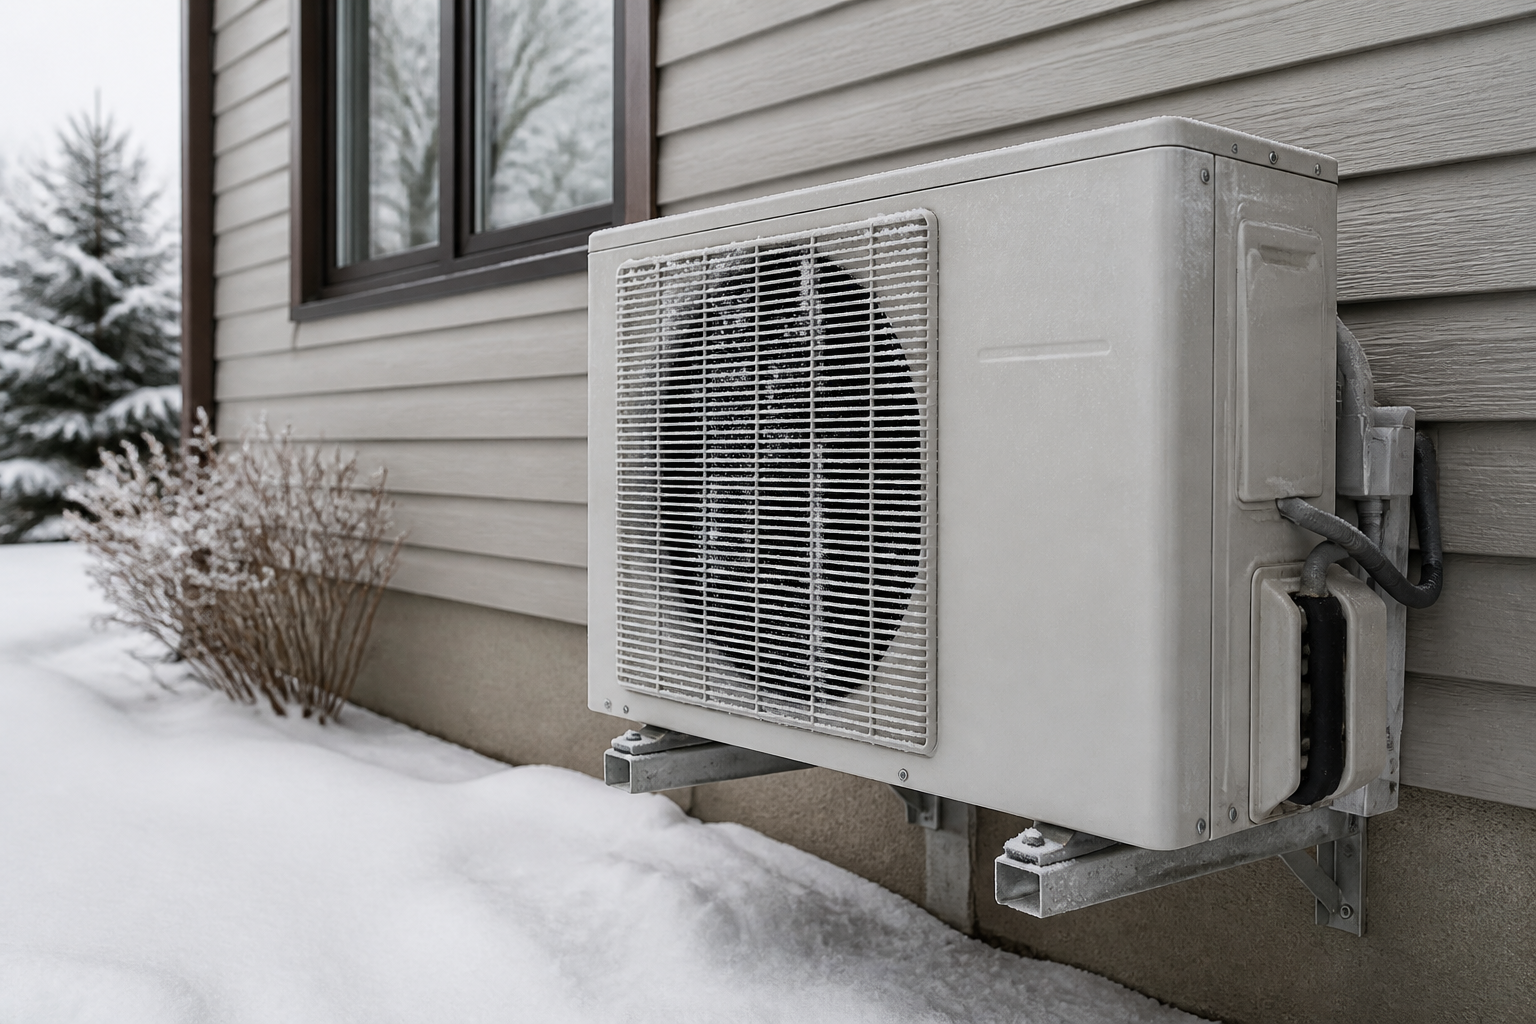
\includegraphics[width=0.58\linewidth]{images/book3/ai/b3-24-heat-pump-winter.png}

{\small \omterm{def:b1:heat-engines:machine}{مضخة حرارية} تأخذ من الهواء في الشتاء: تنتزع الحرارة من الهواء الخارجي البارد وتقدّم للبيت ثلاثة إلى أربعة أضعاف الطاقة الكهربائية التي تستهلكها --- وهي مسألة نهاية الأسبوع.}
\end{omfigure}

\section{مسألة: مضخة البيت الحرارية}

\begin{problem}[{مسألة نهاية الأسبوع --- تدفئة بيت طوال شتاء:
الفاتورة بالمقاومات، وبالغاز، وبمضخة حرارية مثالية، وبأخرى
حقيقية، وأين تذهب كهرباء الحقيقية}]
\label{pb:b1:heat-engines:1}
بيت يفقد الحرارة بالمعدل $K(T_{\mathrm{in}} - T_{\mathrm{out}})$ مع
$K = \qty{250}{W/K}$؛ ويُبقى عند $T_{\mathrm{in}} = \qty{20}{\degreeCelsius}$.
\omterm{def:b1:kinetic-theory:temperature}{ودرجة حرارة} التصميم الخارجية $\qty{-5}{\degreeCelsius}$؛ وموسم التدفئة:
$200$ يوم بمتوسط \omterm{def:b1:kinetic-theory:temperature}{درجة حرارة} خارجية \qty{7}{\degreeCelsius}.
والأسعار: الكهرباء 0.25~\texteuro{} لكل \unit{kW h}، والغاز 0.10~\texteuro{} لكل
\unit{kW h}؛ مع $\qty{1}{kW h} = \qty{3.6}{MJ}$.

\medskip
\noindent\textbf{الجزء I --- البيت والطرائق القديمة.}
\begin{enumerate}
  \item استطاعة التدفئة اللازمة عند \omterm{def:b1:kinetic-theory:temperature}{درجة حرارة} التصميم.
  \item الطاقة اللازمة على امتداد الموسم، بالجول وبوحدة \unit{kW h}.
  \item كلفة الموسم بمقاومات كهربائية.
  \item الكلفة بمِرجل غاز مردوده $0.90$.
  \item تأتي الكهرباء من محطة توليد حرارية مردودها
        $0.40$. فما طاقة الوقود المستهلكة، في الموسم، بالمقاومات
        وبالمِرجل؛ وعلّق على القول إن ``التدفئة الكهربائية مبذّرة
        ترموديناميكيًّا''.
\end{enumerate}

\medskip
\noindent\textbf{الجزء II --- \omterm{def:b1:heat-engines:machine}{المضخة الحرارية} المثالية.}
\begin{enumerate}[resume]
  \item عرّف $e_p$ وبرهن، انطلاقًا من المبدأين على امتداد دور واحد، على أن
        $e_p \leq T_{\mathrm{in}}/(T_{\mathrm{in}} - T_{\mathrm{out}})$.
  \item $e_p$ المثالي عند \omterm{def:b1:kinetic-theory:temperature}{درجة حرارة} التصميم، \omterm{thm:b1:dc-circuits:kirchhoff}{والاستطاعة الكهربائية}
        اللازمة عندئذ.
  \item $e_p$ المثالي عند متوسط \omterm{def:b1:kinetic-theory:temperature}{درجة حرارة} الموسم، ثم (بأخذ تلك
        القيمة للموسم كله) كهرباء الموسم.
  \item فسّر فيزيائيًّا لماذا يهبط $e_p$ حين تهبط \omterm{def:b1:kinetic-theory:temperature}{درجة الحرارة}
        الخارجية، ولماذا يكون ذلك أسوأ سلوك ممكن لجهاز
        تدفئة.
  \item عند نقطة التصميم تسحب المضخة المثالية \qty{0.53}{kW} وتقدّم
        \qty{6.25}{kW}: فمن أين تأتي \qty{5.7}{kW} الباقية،
        ولماذا لا يخرق تبريد الهواء الخارجي البارد لتدفئة بيت دافئ
        المبدأ الثاني؟
\end{enumerate}

\medskip
\noindent\textbf{الجزء III --- الآلة الحقيقية.}
تجري المضخة \omterm{def:b1:heat-engines:vapourcycle}{دور ضغط البخار}. ويتبخر \omterm{def:b1:heat-engines:vapourcycle}{المائع المبرِّد} عند
$T_{\mathrm{ev}} = T_{\mathrm{out}} - \qty{8}{K}$ ويتكثف عند
$T_{\mathrm{cd}} = \qty{313}{K}$ (إذ يجري ماء دارة التدفئة الأرضية عند
\qty{35}{\degreeCelsius})؛ وتبلغ الآلة $0.55$ من قيمة كارنو
المحسوبة بين $T_{\mathrm{ev}}$ و $T_{\mathrm{cd}}$. والحرارة الكامنة
\omterm{def:b1:heat-engines:vapourcycle}{للمائع المبرِّد}: $L = \qty{200}{kJ/kg}$.
\begin{enumerate}[resume]
  \item سمِّ مكوّنات الدور الأربعة، وقل في أيّها يتلقى المائع
        $Q_c$، وفي أيّها يعطي $|Q_h|$ ويتلقى $W$، ولماذا يجب أن يكون
        المبخِّر أبرد من الهواء الخارجي والمكثِّف
        أسخن من البيت.
  \item عند \omterm{def:b1:kinetic-theory:temperature}{درجة حرارة} التصميم: أوجد $T_{\mathrm{ev}}$، ومعامل أداء كارنو $e_p$
        بين $T_{\mathrm{ev}}$ و $T_{\mathrm{cd}}$.
  \item $e_p$ الحقيقي، \omterm{thm:b1:dc-circuits:kirchhoff}{والاستطاعة الكهربائية} المسحوبة، والحرارة المأخوذة من
        الهواء الخارجي، عند \omterm{def:b1:kinetic-theory:temperature}{درجة حرارة} التصميم.
  \item التدفق الكتلي \omterm{def:b1:heat-engines:vapourcycle}{للمائع المبرِّد} عبر المبخِّر.
  \item الأسئلة نفسها ($e_p$ الحقيقي \omterm{thm:b1:dc-circuits:kirchhoff}{والاستطاعة الكهربائية}) عند متوسط
        \omterm{def:b1:kinetic-theory:temperature}{درجة الحرارة} \qty{7}{\degreeCelsius}، حيث يفقد البيت
        \qty{3.25}{kW}.
  \item أعطِ $e_p$ بدلالة $T_{\mathrm{out}}$؛ ثم كهرباء الموسم
        وكلفته، بأخذ $e_p$ عند متوسط \omterm{def:b1:kinetic-theory:temperature}{درجة الحرارة} للموسم كله.
        وقارن بالجزء~I.
  \item طاقة الوقود المستهلكة في محطة التوليد لموسم \omterm{def:b1:heat-engines:machine}{المضخة
        الحرارية}؛ وقارنها بالمقاومات وبالمِرجل.
  \item موجة برد عند \qty{-15}{\degreeCelsius}: أوجد طلب الحرارة، و $e_p$ الحقيقي،
        \omterm{thm:b1:dc-circuits:kirchhoff}{والاستطاعة الكهربائية} لو استطاعت المضخة تقديمه. وسعة الضاغط
        تهبط فعليًّا مع $T_{\mathrm{ev}}$ فلا تستطيع المضخة أن
        تقدّم هناك إلا \qty{3.8}{kW}: فما استطاعة المقاومة الاحتياطية اللازمة، وما
        معنى ``تحديد قياس \omterm{def:b1:heat-engines:machine}{مضخة حرارية}''؟
  \item ولو كانت في البيت مشعّات قديمة تحتاج إلى ماء عند
        \qty{60}{\degreeCelsius} ($T_{\mathrm{cd}} = \qty{338}{K}$): فما $e_p$ الحقيقي
        \omterm{thm:b1:dc-circuits:kirchhoff}{والاستطاعة الكهربائية} عند \omterm{def:b1:kinetic-theory:temperature}{درجة حرارة} التصميم؛ واستنتج ما يخصّ
        اختيار أجهزة البثّ الحراري.
\end{enumerate}

\medskip
\noindent\textbf{الجزء IV --- أين تذهب الكهرباء.}
\begin{enumerate}[resume]
  \item بيّن أنه من أجل \omterm{def:b1:heat-engines:machine}{مضخة حرارية} تقدّم $|Q_h|$ للبيت عند
        $T_{\mathrm{in}}$ من هواء خارجي عند $T_{\mathrm{out}}$، يكون
        $W = |Q_h|(1 - T_{\mathrm{out}}/T_{\mathrm{in}}) + T_{\mathrm{out}}S_{\mathrm{created}}$.
  \item عند نقطة التصميم، ما الإنتروبيا المُنشأة في الثانية بنقل
        الحرارة عبر المكثِّف (من \qty{313}{K} إلى البيت)
        وعبر المبخِّر (من الهواء الخارجي إلى \qty{260}{K})؟
  \item ما \omterm{thm:b1:dc-circuits:kirchhoff}{الاستطاعة الكهربائية} التي يكلّفها هذان الفرقان؛ وما نسبتها من
        \qty{1.92}{kW} المسحوبة؟
  \item الإنتروبيا الكلية المُنشأة في الثانية بالآلة الحقيقية (قارن
        \qty{1.92}{kW} التي تسحبها بالمقدار \qty{0.53}{kW} المثالي)؛ ونصيب
        المبادلين؛ وسمِّ المنابع الأخرى.
  \item نصّف الفرقين (\qty{4}{K} و\qty{10}{K}): فما الإنتروبيا المُنشأة
        في المبادلين \omterm{thm:b1:dc-circuits:kirchhoff}{والاستطاعة الكهربائية} الموفَّرة؛ وما الذي يكلّفه تنصيف
        فرق للمصمِّم؟
  \item لخّص في ثلاثة أعداد: كيلوواط ساعي من الحرارة لكل
        كيلوواط ساعي من الكهرباء على امتداد الموسم؛ وكلفة الموسم
        مقابل الغاز؛ ثم، مع كهرباء تُطلق \qty{60}{g} من CO$_2$ لكل
        \unit{kW h} وغاز يطلق \qty{200}{g}، ما الكربون الذي يطلقه كل
        مسلك.
\end{enumerate}
\end{problem}
